\documentclass[xcolor=x11names,compress]{beamer}
\usepackage[english]{babel}

%% General document %%%%%%%%%%%%%%%%%%%%%%%%%%%%%%%%%%
\usepackage{graphicx}
\usepackage{tikz}
\usetikzlibrary{decorations.fractals}
%%%%%%%%%%%%%%%%%%%%%%%%%%%%%%%%%%%%%%%%%%%%%%%%%%%%%%


%% Beamer Layout %%%%%%%%%%%%%%%%%%%%%%%%%%%%%%%%%%
\useoutertheme[subsection=false,shadow]{miniframes}
\useinnertheme{default}
\usefonttheme{serif}
\usepackage{palatino}

\setbeamerfont{title like}{shape=\scshape}
\setbeamerfont{frametitle}{shape=\scshape}

\setbeamercolor*{lower separation line head}{bg=DeepSkyBlue4} 
\setbeamercolor*{normal text}{fg=black,bg=white} 
\setbeamercolor*{alerted text}{fg=red} 
\setbeamercolor*{example text}{fg=black} 
\setbeamercolor*{structure}{fg=black} 
 
\setbeamercolor*{palette tertiary}{fg=black,bg=black!10} 
\setbeamercolor*{palette quaternary}{fg=black,bg=black!10} 

\renewcommand{\(}{\begin{columns}}
\renewcommand{\)}{\end{columns}}
\newcommand{\<}[1]{\begin{column}{#1}}
\renewcommand{\>}{\end{column}}
%%%%%%%%%%%%%%%%%%%%%%%%%%%%%%%%%%%%%%%%%%%%%%%%%%



%\usepackage[english]{babel}
\usepackage[utf8]{inputenc}
%\usetheme{Goettingen}

\begin{document}
\title{Bifurcations in continuous time dynamical systems}
\author{Debsankha Manik}

\begin{frame}

%opening

\titlepage

\end{frame}



\section{Scenarios}
\begin{frame}{Definitions}
A simple piecewise smooth function:
\begin{displaymath}
   \dot{\bf{x}} = \left\{
     \begin{array}{lr}
       F_1(\bf{x}) & : H(\bf{x})<0\\
       F_2(\bf{x}) & : H(\bf{x})>0
     \end{array}
   \right.
\end{displaymath}

$H(\bf{x})=$The boundary.  \\


The flows of $F_1$ and $F_2$ are $\varphi_1(x)$ and $\varphi_2(x)$ 
respectively, defined in respective regions and also in the neighbourhood of 
the boundary.  


\end{frame}

\begin{frame}
\begin{figure}
\caption{Possible scenarios}
\begin{center}
\includegraphics[height=0.9\textheight]{c-bifs}
\end{center}
\end{figure}

\end{frame}

\section{Bifurcation of equillibria}

\begin{frame}
Choose a coordinate system such that:\\
\begin{displaymath}
   \dot{\bf{x}} = \left\{
     \begin{array}{lr}
       F_1(\bf{x}) & : x_n<0\\
       F_2(\bf{x}) & : x_n>0
     \end{array}
   \right.
\end{displaymath}

and $\bf{x}=0$ is a grazing point.  

$x_n==n$th component of $\bf{x}$.  \\

Locally linearize:
\begin{displaymath}
   \dot{\bf{x}} = \left\{
     \begin{array}{lr}
       \bf{A_1x+\bf{B}\mu} & : x_n<0\\
       \bf{A_2x+\bf{B}\mu} & : x_n<0\\
     \end{array}
   \right.
\end{displaymath}

Where:\\
\[
\bf{A_i}=\frac{\partial F_1}{\partial \bf{x}}_{x=0}
\]
and 
$\bf{B}=\frac{\partial F_1}{\partial \mu}_{\mu=0}=\frac{\partial F_2}{\partial \mu}_{\mu=0}$
 (Due to continuity).

Also, $\bf{A_1}$ and $\bf{A_2}$ can differ only in the $n-$th column (Again due to continuity).


\end{frame}


\begin{frame}
Let:\\
$A_1\bf{x}^*_1+\bf{B}\mu=0$,
$A_2\bf{x}^*_2+\bf{B}\mu=0$.  


Assuming $A_i$'s are invertible:
\[
\bf{x}^*_i=-\bf{A_i}^{-1}\bf{B}\mu=-\frac{adj(\bf{A_i})}{det(\bf{A_i})}\bf{B}\mu
\]

The solutions exist iff:
\[
x^*_{1_{n<0}}<0, x^*_{2{_n}}>0. 
\]  

Now, 
\[
x^*_{1_k}=\frac{c^*_{1_k}}{det(\bf{A_1})}\mu, x^*_{2_k}=\frac{c^*_{2_k}}{det(\bf{A_2})}
\]

Where, \[
c^*_{i_k}=[-adj(\bf{A_i)B}]_k
\]

Because $A_1$ differs from $A_2$ only in $n-$th column, $c^*_{1_n}=c^*_{2_n}:=C$

\end{frame}


\begin{frame}{Condition for border crossing of equillibria}
Note:\\
\[
x^*_{1_n}=\frac{c}{det(\bf{A_1})}\mu, x^*_{2_k}=\frac{c}{det(\bf{A_2})}\mu
\]

{\bf Cases:}\\
\begin{enumerate}
\item $det({\bf A_1})det({\bf A_1})<0$.  $x^*_{1_n}$ and $x^*_{2_n}$ always have 
opposite signs.  \\
\item $det({\bf A_1})det({\bf A_1})>0$.  $x^*_{1_n}$ and $x^*_{2_n}$ always have 
same signs.  
\end{enumerate}

\begin{figure}
\begin{center}
\includegraphics[width=0.9\columnwidth]{cases}
\end{center}
\end{figure}

\end{frame}


\section{Grazing}

\begin{frame}{Grazing}

\begin{figure}
\caption{}
\begin{center}
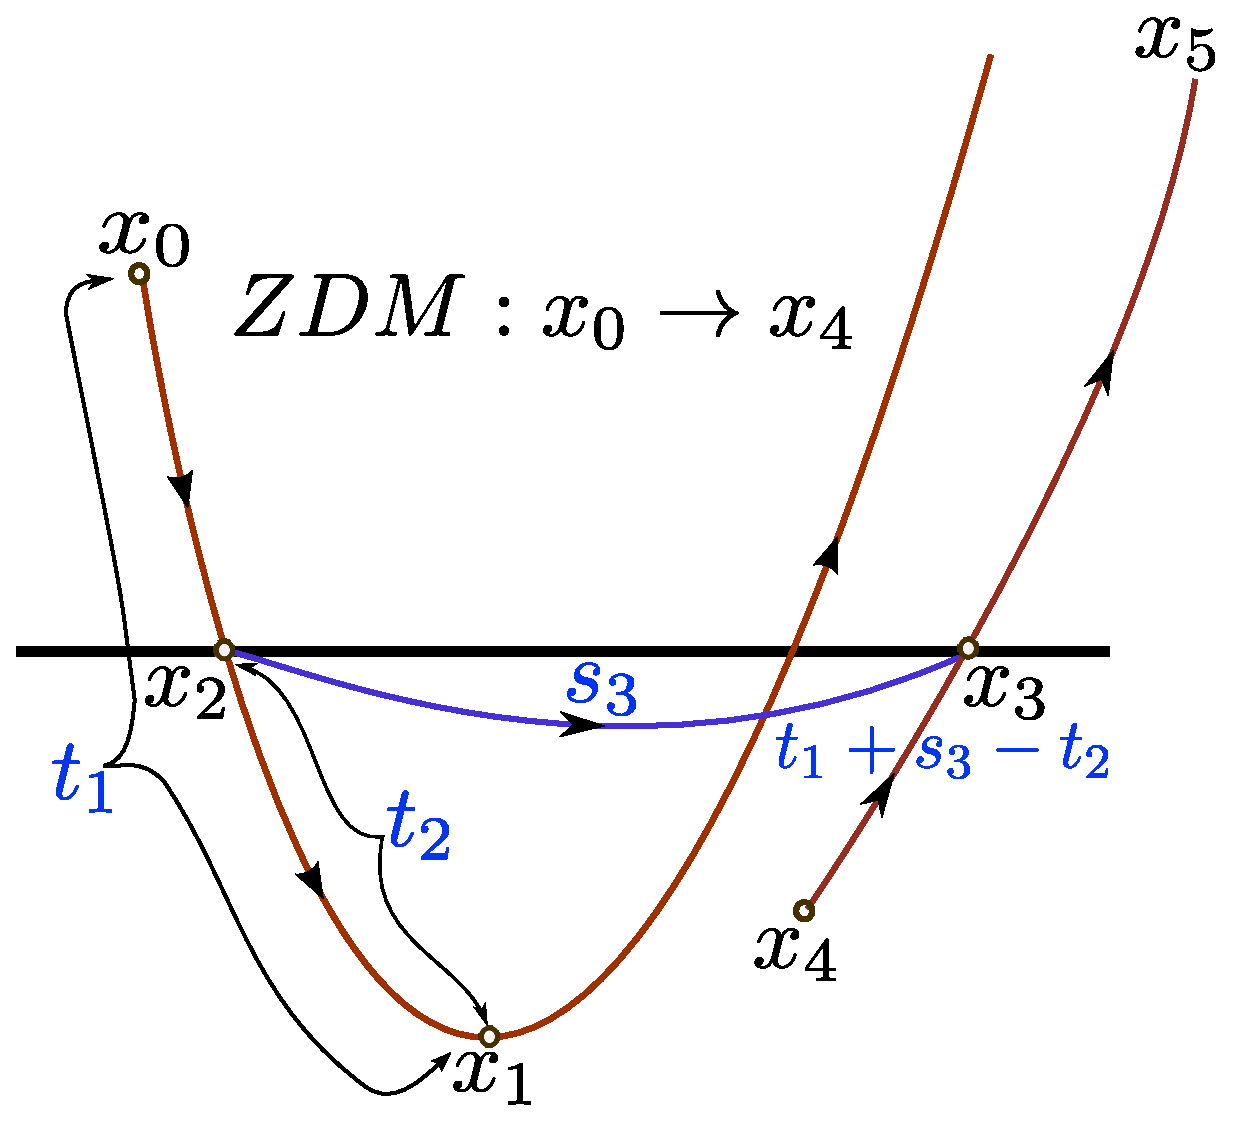
\includegraphics[height=0.7\textheight]{ZDM}
\end{center}
\end{figure}
\end{frame}



\begin{frame}{How to get the ZDM?}

{\bf Why ZDM?}\\
Consider a Poincare section $t mod T=0$. Then the Poincare map would be 
simplified to:\\
\[
f(x_n)=\varphi_2(ZDM(\varphi_1(x_n,\tau)),T-\tau)
\] 


\begin{itemize}
\item $t_1$ == time for $x_0$ to $x_1$
\item $t_2$ == time for $x_2$ to $x_1$
\item $s_3$ == time for $x_2$ to $x_3$
\end{itemize}

\begin{enumerate}
\item Solve for: $T_1(x)$ given by:\[
E_1(x,T_1)=\frac{dH}{dt}|_{t=T_1}=0, T_1(0)=0.
\]
$t_1=T_1(x_0)$
\item Solve for $E_2(x,y,T_2)$ given by:
\[
T_2\sqrt{\frac{H(\varphi_1(x,T_1(x)-T_2))-H(\varphi_1(x,T_1(x)))}{T_2^2}}-y=0
\]
$t_2=T_2(x_0,\sqrt(-H_{min}(x_0)))$

\end{enumerate}

\end{frame}

\begin{frame}
\begin{enumerate}
\item Solve for \[
E_3(x,S_3)=\frac{H(\varphi_2(x,s_3))-H(x)}{s_3}=0
\]
$s_3=S_3(x_2)$
\end{enumerate}

\end{frame}






\end{document}
